\documentclass[
  bibliography=totoc,     % Literatur im Inhaltsverzeichnis
  captions=tableheading,  % Tabellenüberschriften
  titlepage=firstiscover, % Titelseite ist Deckblatt
]{scrartcl}

% Paket float verbessern
\usepackage{scrhack}

% Warnung, falls nochmal kompiliert werden muss
\usepackage[aux]{rerunfilecheck}

% unverzichtbare Mathe-Befehle
\usepackage{amsmath}
% viele Mathe-Symbole
\usepackage{amssymb}
% Erweiterungen für amsmath
\usepackage{mathtools}

% Fonteinstellungen
\usepackage{fontspec}
\usepackage{colortbl}
% Latin Modern Fonts werden automatisch geladen
% Alternativ zum Beispiel:
%\setromanfont{Libertinus Serif}
%\setsansfont{Libertinus Sans}
%\setmonofont{Libertinus Mono}

% Wenn man andere Schriftarten gesetzt hat,
% sollte man das Seiten-Layout neu berechnen lassen
\recalctypearea{}

% deutsche Spracheinstellungen
\usepackage{polyglossia}
\setmainlanguage{german}


\usepackage[
  math-style=ISO,    % ┐
  bold-style=ISO,    % │
  sans-style=italic, % │ ISO-Standard folgen
  nabla=upright,     % │
  partial=upright,   % ┘
  warnings-off={           % ┐
    mathtools-colon,       % │ unnötige Warnungen ausschalten
    mathtools-overbracket, % │
  },                       % ┘
]{unicode-math}

% traditionelle Fonts für Mathematik
\setmathfont{Latin Modern Math}
% Alternativ zum Beispiel:
%\setmathfont{Libertinus Math}

\setmathfont{XITS Math}[range={scr, bfscr}]
\setmathfont{XITS Math}[range={cal, bfcal}, StylisticSet=1]

% Zahlen und Einheiten
\usepackage[
  locale=DE,                   % deutsche Einstellungen
  separate-uncertainty=true,   % immer Fehler mit \pm
  per-mode=symbol-or-fraction, % / in inline math, fraction in display math
]{siunitx}

% chemische Formeln
\usepackage[
  version=4,
  math-greek=default, % ┐ mit unicode-math zusammenarbeiten
  text-greek=default, % ┘
]{mhchem}

% richtige Anführungszeichen
\usepackage[autostyle]{csquotes}

% schöne Brüche im Text
\usepackage{xfrac}

% Standardplatzierung für Floats einstellen
\usepackage{float}
\floatplacement{figure}{htbp}
\floatplacement{table}{htbp}

% Floats innerhalb einer Section halten
\usepackage[
  section, % Floats innerhalb der Section halten
  below,   % unterhalb der Section aber auf der selben Seite ist ok
]{placeins}

% Seite drehen für breite Tabellen: landscape Umgebung
\usepackage{pdflscape}

% Captions schöner machen.
\usepackage[
  labelfont=bf,        % Tabelle x: Abbildung y: ist jetzt fett
  font=small,          % Schrift etwas kleiner als Dokument
  width=0.9\textwidth, % maximale Breite einer Caption schmaler
]{caption}
% subfigure, subtable, subref
\usepackage{subcaption}

% Grafiken können eingebunden werden
\usepackage{graphicx}
% größere Variation von Dateinamen möglich
\usepackage{grffile}

% schöne Tabellen
\usepackage{booktabs}

% Verbesserungen am Schriftbild
\usepackage{microtype}

% Literaturverzeichnis
\usepackage[
  backend=biber,
]{biblatex}
% Quellendatenbank
\addbibresource{lit.bib}
%\addbibresource{programme.bib}

% Hyperlinks im Dokument
\usepackage[
  unicode,        % Unicode in PDF-Attributen erlauben
  pdfusetitle,    % Titel, Autoren und Datum als PDF-Attribute
  pdfcreator={},  % ┐ PDF-Attribute säubern
  pdfproducer={}, % ┘
]{hyperref}
% erweiterte Bookmarks im PDF
\usepackage{bookmark}

% Trennung von Wörtern mit Strichen
\usepackage[shortcuts]{extdash}

\author{%
  AUTOR A\\%
  \href{mailto:authorA@udo.edu}{authorA@udo.edu}%
  \texorpdfstring{\and}{,}%
  AUTOR B\\%
  \href{mailto:authorB@udo.edu}{authorB@udo.edu}%
}
\publishers{TU Dortmund – Fakultät Physik}


\usepackage{fancyhdr}
\pagestyle{fancy}
\fancyhead{}
\fancyfoot{}
\renewcommand{\headrulewidth}{0pt}
\fancyfoot[R]{\thepage}

\title{Versuch 504 Thermische Elektronenemission}
\author{
  Robert Konradi\\%
  \href{mailto:authorA@udo.edu}{robert.konradi@tu-dortmund.de}%
  \texorpdfstring{\and}{,}%
  Lauritz Klünder\\%
  \href{mailto:authorB@udo.edu}{lauritz.kluender@tu-dortmund.de}%
}
\date{Durchführung: 26.06.2018, Abgabe: 03.07.2018}
\publishers{TU Dortmund – Fakultät Physik}
\begin{document}
\maketitle
\setlength{\parindent}{0pt}
\thispagestyle{empty}
\tableofcontents
\newpage
\section{Zielsetzung}
In diesem Versuch sollen die Grundlagen der Ultraschallechographie
in ihren Anwedungsbereichen kennengelernt werden.
\section{Theorie}
Als Ultraschall bezeichnet man den Frequenzbereich von 20 kHz bis ca. 1 GHz.
Zum Vergleich hören Menschen ein Frequenzbereich von 16 Hz bis ca. 20 kHz.
Um diese longitudinalen Wellen, in seinen Anwedungen, wie in der Werkstoffprüfung
und in der Medizin, beschreiben zu können wird diese Formel
\begin{equation*}
  p(x,t)= p_0 + v_0 Z cos(\omega t - k x)
\end{equation*}
verwendet.
Dabei ist $Z = c* \rho$ die akustische Impedanz und $\rho$ ist die Dichte des durchstrahlten Materials.
Da Ultraschall sich aufgrund von Druckschankungen fortbewegt, ist ihre Geschwindigkeit materialabhängig.
Die Schallgeschwindigkeit in einer Flüssigkeit ist von ihrer Kompressibilität $\kappa$ und der Dichte $\rho$
abhängig.
\begin{equation*}
  c_{\text{flüssig}} = \sqrt{\frac{1}{\kappa \cdot \rho}}
\end{equation*}
Bei Schallausbreitung in Festkörpern sind auch Transversalwellen möglich, da sie Richtungsabhängig sind.
Hierbei ist die Kompressibilität $\kappa$ antiproprtional zum Elastizitätsmodul $E$ des Festkörpers.
\begin{equation*}
  c_{\text{fest}} = \sqrt{\frac{E}{\rho}}
\end{equation*}
Die Intensität einer Schallwelle nimmt exponentiell ab.
\begin{equation}
  I(x) =I_0 \cdot e^{-\alpha x}
  \label{eq:4}
\end{equation}
Dabei  ist$\alpha$ der Absorptionskoeffizient der Schallamplitude.
Da Luft ein sehr hohen Absorptionskoeffizient hat wird in der Medizin ein Kontaktmittel
zwischen Sonde und dem untersuchendem Material verwendet.
Wie bei elektromagnetische Wellen haben sie die Eigenschaft zu reflektieren.
Dabei setzt sich der Reflexionskoeffizient R, das Verhältnis von reflektierten zu einfallender Schallintensität zusammen.
\begin{equation*}
  R = \left(\frac{Z_1 - Z_2} {Z_1 + Z_2}\right)^2
\end{equation*}
Der Anteil der transmittierten Wellen lässt sich aus $T=1-R$ berechnen.
Um Ultraschallwellen zu erzeugen nutzt man den piezo-elektrischen Effekt aus.
Dabei werden die piezoelektrische Kristall in ein elektrisches Wechselfeld gebracht.
Durch die Richtung des elektrischen Feldes werden die polaren Achsen des Kristalls zu Schwingung angeregt und
senden dabei Ultraschallwellen aus.
In der Medizin werden zwei Messmethoden angewendet.
Zum einen das Durchschallungs-Verfahren. Wie der Name schon sagt werden die Probestücke durchschallt. Dabei sendet
der Sender ein kurzeitigen Schallimpuls aus und am andere Ende wird dies durch ein Empfänger aufgefangen.
Bei einer Fehlstelle wird die Intensität abgeschwächte am Empfänger gemessen.
Die andere Messmethode ist das Impuls-Echo-Verfahren. Dabei ist der Sender gleichzeitig der Empfänger. Bei bekannter Schallgeschwindigkeit
lässt sich die zurückgelegte Strecke des Ultraschalls mit folgender Formel bestimmen:
\begin{equation}
  s=\frac{1}{2} c t.
  \label{eq:6}
\end{equation}
Bei einer Fehlstelle wird der reflektierte Schall eher am Empfänger angekommen.
Die Laufzeitdiagramme können in einen A- oder B-Scan dargestellt werden.

\section{Durchführung}

\subsection{Elektronenstrahl im elektrischen Feld}

In diesem Versuch wird zunächst die Proportionalität zwischen $D$ und $U_d$
überprüft bei fünf verschiedenen Beschleunigungsspannungen. Dabei wird die Schaltung
verwendet die in Abbildung \ref{abb:3} dargestellt ist.

\begin{figure}[H]
  \centering
  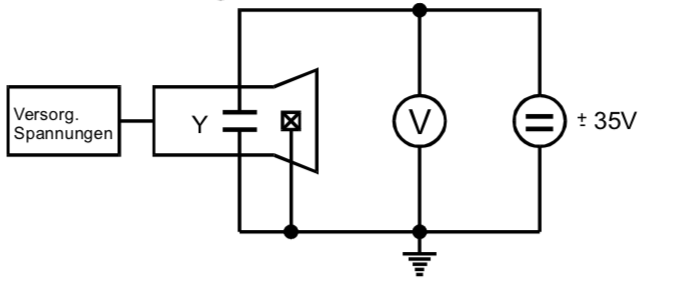
\includegraphics[width=\textwidth]{content/Schaltung1.png}
  \caption{Schaltung zur Bestimmung der Proportionalität von $D$ und $U_d$ \cite{1}.}
  \label{abb:3}
\end{figure}

Daraufhin wird durch Anschließen einer Sägezahnspannung und einer Sinusspannung an
der Kathodenstrahlröhre ein Oszillograph hergestellt. Durch Variation der Sägezahnfrequenz
werden vier verschiedene Frequenzen bestimmt, bei denen ein stehendes Bild der Sinusspannung
zu sehen ist, bei denen also Gleichung \ref{eq:2} erfüllt ist. Dabei wird die Schaltung, die in
Abbildung \ref{abb:4} gezeigt ist verwendet.

\begin{figure}[H]
  \centering
  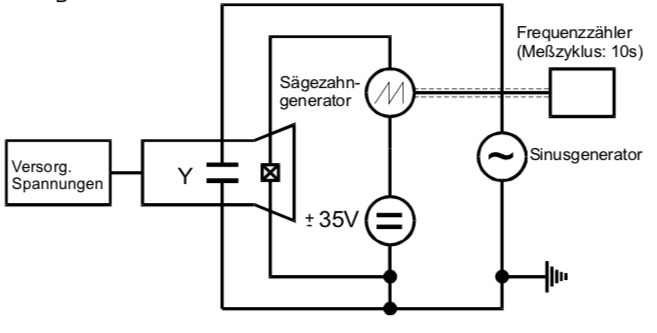
\includegraphics[width=\textwidth]{content/Schaltung2.png}
  \caption{Schaltung für einen Kathodenstrahl-Oszillographen \cite{1}.}
  \label{abb:4}
\end{figure}

\subsection{Elektronenstrahl im transversalen Magnetfeld}

Bei diesem Versuch wird zunächst die Ablenkung von Elektronen durch ein nahezu homogenes
Magnetfeld bestimmt. Dazu wird eine Helmholtz-Spule verwendet. Das Magnetfeld dieser
Spule lässt sich mit folgender Gleichung bestimmen

\begin{equation}
  B = \mu_0 \frac{8 N I}{\sqrt{125} R}.
  \label{eq:4}
\end{equation}

Dabei ist $N$ die Windungszahl, $I$ der Spulenstrom, $R$ der Spulenradius und
$\mu_0$ ist die magnetische Feldkonstante.

Nun wird die Strahlenverschiebung $D$ in Abhängigkeit von dem Magnetfeld $B$, was von der
Helmholtz-Spule erzeugt wird, für verschiedene
Beschleunigungsspannungen gemessen.

Daraufhin wird noch das lokale Erdmagnetfeld bestimmt. Dazu wird die Kathodenstrahlröhre
in Nord-Süd-Richtung ausgerichtet. Dann wird die Röhre in Ost-West-Richtung gedreht.
Danach wird das Magnetfeld der Helmholtz-Spule eingeschaltet und so hoch gedreht, dass
die Strahlenverschiebung durch das Erdmagnetfeld kompensiert wird. Dieses Magnetfeld ist dann
die Horizontalkomponente des Magnetfeldes $B_\text{hor}$.
Zur Bestimmung von $B_\text{total}$ wird nun noch der Inklinationswinkel $\varphi$
bestimmt. Das ist der Winkel zwischen Horizontalebene und Richtung des Erdmagnetfeldes. Dazu wird
ein Kompass in der horizontalen Ebene der Kathodenstrahlröhre in Nord-Süd-Richtung ausgerichtet
und dann um $90°$ geschwenkt. Dann zeigt der Kompass $\varphi$ an.


In der Abbildung \ref{abb:5} sind die Abmessungen der Kathodenstrahlröhre dargestellt.

\begin{figure}[H]
  \centering
  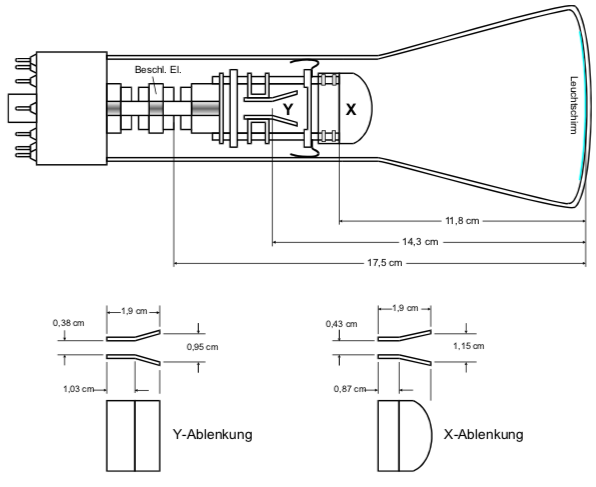
\includegraphics[width=\textwidth]{content/Roehre.png}
  \caption{Konstruktionszeichnung der Kathodenstrahlröhre \cite{1}.}
  \label{abb:5}
\end{figure}

\section{Auswertung}
\subsection{Vorbereitung}
Die Literaturwerte der charakteristischen Röntgenstrahlung von Kupfer und die zugehörigen
Glanzwinkel $\theta$ sind \cite{2}:
\begin{itemize}
  \item $\text{Cu-}K_\alpha \text{-Linie} = 8,048 \,\text{keV} , \, \, \theta_\alpha = 22.49^\circ$
  \item $\text{Cu-}K_\beta \text{-Linie} = 8,905 \,\text{keV} , \, \, \theta_\beta = 20,22^\circ$

\end{itemize}

Des Weiteren sind die Literaturwerte der K-Kante von verschiedenen Materialien und die zugehörigen
Braggwinkel $\theta$ sowie die Abschirmkonstante $\sigma_k$ in der Tabelle (\ref{tab:1}) aufgelistet.
\begin{table}
  \centering
  \caption{Eigenschaftendarstellung der Materialien \cite{3}.}
  \label{tab:1}
  \begin{tabular}{c c c c c}
    \toprule
     & $Z$ & $E_{lit}\,/ \, \text{keV}$ &$\theta_{lit}\,/\,\circ$ & $\sigma_k$ \\
    \midrule
    Zn & 30 & 9,65  &  18.6 & 3.56 \\
    Ge & 32 & 11,1  &  16,1 & 3,43 \\
    Br & 35 & 13,47 &  13,2 & 3,53 \\
    Rb & 37 & 15,2  &  11,6 & 3,57 \\
    Sr & 38 & 16,1  &  11   & 3,59 \\
    Zr & 40 & 17,99 &  9,85 & 3,63 \\
    Nb & 41 & 18,98 &  9,33 & 3,64 \\
    \bottomrule
  \end{tabular}
\end{table}

\subsection{Überprüfung der Bragg Bedingung}
Es werden die Voreinstellungen die in der Durchführung angesprochen worden sind
durchgeführt und die Ergebnisse in der Tabelle (\ref{tab:2})
dargestellt als auch in der Abbildung (\ref{Bild:1})

\begin{table}[H]
  \centering
  \caption{Darstellung der Messreihe bei einer Zählrohwinkelrate bei 35 kV.}
  \label{tab:2}
  \begin{tabular}{c c c c}
  \toprule
  $2\cdot\theta \, / \, \circ$&	$I \, / \, \text{Imp/s}$ &$2\cdot\theta \, / \, \circ$&	$I \, / \, \text{imp/s}$ \\
  \midrule
  26,0&	31,0 &  28,1 &	156,0 \\
  26,1&	33,0 &  28,2 &  152,0 \\
  26,2&	42,0 &  28,3 &  150,0 \\
  26,3&	47,0 &  28,4 &  152,0 \\
  26,4&	48,0 &  28,5 &  138,0 \\
  26,5&	51,0 &  28,6 &  130,0 \\
  26,6&	58,0 &  28,7 &  126,0 \\
  26,7&	63,0 &  28,8 &  115,0 \\
  26,8&	60,0 &  28,9 &   97,0 \\
  26,9&	87,0 &  29,0 &   92,0 \\
  27,0&	84,0 &  29,1 &   88,0 \\
  27,1&	93,0 &  29,2 &   73,0 \\
  27,2&	100,0&  29,3 &   58,0 \\
  27,3&	112,0&  29,4 &   53,0 \\
  27,4&	113,0&  29,5 &   42,0 \\
  27,5&	116,0&  29,6 &   38,0 \\
  27,6&	117,0&  29,7 &   30,0 \\
  27,7&	132,0&  29,8 &   26,0 \\
  27,8&	136,0&  29,9 &   33,0 \\
  27,9&	137,0&  30,0 &   35,0 \\
  28,0&	147,0&    -  &     -  \\
 \bottomrule
\end{tabular}
\end{table}
Der Sollwinkel liegt bei $28^\circ$. Die aufgezeichnete Messreihe zeigen ein Maximum bei $28,1^\circ$.
Die Abweichung beträgt $0,1^\circ$ ($\approx 0,36\%$) und liegt im Toleranzbereich.

\subsection{Emissionsspektrum der Cu-Röntgenröhre}
Zur Aufnahme für das Emissionsspektrum wird der Koppelmodus 2:1 aktiviert. Im Anhang unter der Abbildung (\ref{Bild:2})
sind die Messergebnisse graphisch dargestellt. Zudem zeigen sie einen Bremsberg als auch die
$K_\beta \text{-Linie}$ und die $K_\alpha \text{-Linie}$ an.

Aus dem Grenzwinkel $\theta$ wird die minimale Wellenlänge bzw. die maximale Energie bestimmt.
Mit der Formel (\ref{eq:5}) und einer Gitterkonstante von $d=201,4 pm$  ist die minimale Wellenlänge bei
\begin{equation*}
  \lambda_{\text{min}} = \num{3.811e-11} \text{m}
\end{equation*}
Mit der Formel (\ref{eq:1}) ist die dazugehörige maximale Energie bei
\begin{equation*}
  E_{\text{max}} = \num{5.212e-15} \text{J} = 32,53 \, \text{keV}
\end{equation*}
Der erwartete Wert soll bei $E = 35 \,\text{keV}$ liegen.
Damit ist die Abweichung bei $7,06 \%$.\\

Mit der Full Width at Half Maximum Methode wird die Energieauflösung der $K_\alpha \text{- und der} \, K_\beta \text{-Linien}$ in Abbildung (\ref{Bild:2}) bestimmt.\\
Für $K_\beta$ folgt:
\begin{itemize}
  \item $\theta_1 = 39,52^\circ \Rightarrow E_1 = 9,1 \, \text{keV}$
  \item $\theta_2 = 40,95^\circ \Rightarrow E_2 = 8,8 \, \text{keV}$
\end{itemize}
Für die Umrechnung vom Braggwinkel zur Energie werden die Formelen (\ref{eq:5}) und (\ref{eq:1}) benutzt.
Die Energiedifferenz $\Delta E = E_1 - E_2 = 0,3 \, \text{keV}$ ist die gesuchte Energieauflösung.\\

Für $K_\alpha$ folgt:
\begin{itemize}
  \item $\theta_1 = 44,05^\circ \Rightarrow E_1 = 8,2 \, \text{keV}$
  \item $\theta_2 = 45,24^\circ \Rightarrow E_2 = 8 \, \text{keV}$
\end{itemize}
Die Energiedifferenz hier ist bei $\Delta E = 0,2 \,\text{keV}$ und die gesuchte Energieauflösung.

Anschließend werden die Abschirmkonstanten für $K_\alpha$ und für $K_\beta$ bestimmt.
Zunächst werden die Energie der $K_\beta \, \text{-und}\, K_\alpha$ -Peaks von Abbildung (\ref{Bild:2}) bestimmt.
Die folgende Umrechnung ist die selbe wie oben.
\begin{itemize}
  \item $\theta_\alpha = 44,52^\circ \Rightarrow E_\alpha = 8,13 \,\text{keV}$
  \item $\theta_\beta = 40,24^\circ \Rightarrow E_\beta = 8,95 \,\text{keV}$
\end{itemize}
Die Energiedifferenz der beiden Absorptionsenergien ist $\Delta E = 0,82 \, \text{keV}$
Durch Einsetzen in die Gleichung (\ref{eq:2}) folgt
\begin{equation*}
  \Delta E = R_\infty \cdot (z_{cu} - \sigma)^2 \cdot [(\frac{1}{1^2}-\frac{1}{2^2})-(\frac{1}{1^2}-\frac{1}{3^2})]
\end{equation*}
Durch umstellen und einsetzen der Werte ergibt sich für $\sigma$:
\begin{equation*}
  \sigma = z_{cu} - \sqrt{\frac{\Delta E \cdot 36}{R_\infty \cdot 5}} = 9,17
\end{equation*}

\subsection{Absorptionsspektrum}
Für diesen Versuchsteil werden folgende Absorber benutzt: Brom (Br), Strontium (Sr) und Zirkonium (Zr).
Die jeweiligen Ergebnisse zu den Messreihen sind unter Anhang graphisch dargestellt.
\subsubsection{Brom}
Aus der Absorptionskurve in Abbildung (\ref{Bild:3}) kann folgender Winkel abgelesen werden und mit der Formel (\ref{eq:5}) und (\ref{eq:1}) die
Absorptionsenergie bestimmt werden
\begin{itemize}
  \item $\theta_{Br} = 13,3^\circ \Rightarrow E_{Br} = 13,38 \, \text{keV}$
\end{itemize}
Nun wird nach der Formel (\ref{eq:2}) die Abschirmkonstante $\sigma_{br}$ bestimmt.
\begin{itemize}
  \item $\sigma_{Br} = Z_{Br} - \sqrt{\frac{E_{Br}}{R_\infty}} = 3,63$
\end{itemize}
\subsubsection{Strontium}
Aus der Absorptionskurve in Abbildung (\ref{Bild:4}) kann folgender Winkel abgelesen werden und mit der Formel (\ref{eq:5}) und (\ref{eq:1}) die
Absorptionsenergie bestimmt werden
\begin{itemize}
  \item $\theta_{Sr} = 11,1^\circ \Rightarrow E_{Sr} = 15,99 \,\text{keV}$
\end{itemize}
Nun wird nach der Formel (\ref{eq:2}) die Abschirmkonstante $\sigma_{Sr}$ bestimmt.
\begin{itemize}
  \item $\sigma_{Sr} = Z_{Sr} - \sqrt{\frac{E_{Sr}}{R_\infty}} = 3,71$
\end{itemize}
\subsubsection{Zirkonium}
Aus der Absorptionskurve in Abbildung (\ref{Bild:5}) kann folgender Winkel abgelesen werden und mit der Formel (\ref{eq:5}) und (\ref{eq:1}) die
Absorptionsenergie bestimmt werden
\begin{itemize}
  \item $\theta_{Zr} = 10,19^\circ \Rightarrow E_{Zr} = 17,4 \, \text{keV}$
\end{itemize}
Nun wird nach der Formel (\ref{eq:2}) die Abschirmkonstante $\sigma_{Zr}$ bestimmt.
\begin{itemize}
  \item $\sigma_{Zr} = Z_{Zr} - \sqrt{\frac{E_{Zr}}{R_\infty}} = 4,23$
\end{itemize}

Nach dem Moseleyschen Gesetz ist die Absorptionsenergie $E_n$ proportional zu Z$^2$ siehe Formel (\ref{eq:2}).
Zur Bestimmung der Rydbergenergie $R_\infty$ wird sie umgeformt zu:
\begin{equation*}
  \sqrt{E_n} = \sqrt{R_\infty} \cdot Z - \sqrt{R_\infty} \cdot \sigma
\end{equation*}
Zu sehen ist eine lineare Gleichung mit der $\sqrt{R_\infty}$ als Steigung m und $\sqrt{R_\infty} \cdot \sigma$ als
y-Achsenschnitt b.
In Abbildung (\ref{abb:3}) sind die Messergebnisse graphisch dargestellt und mit Python 3.6.4 wurde
die Regressionsgerade berechnet.
\begin{figure}[H]
  \centering
  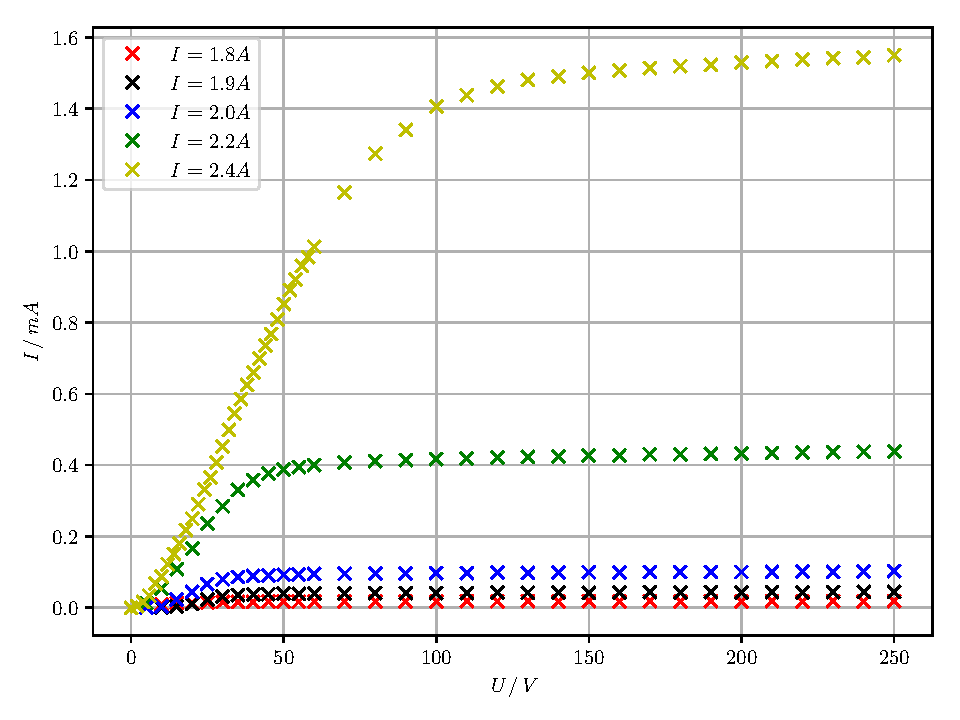
\includegraphics[width=\textwidth]{plot1.pdf}
  \caption{Graphische Darstellung zur Bestimmung der Rydbergenergie.}
  \label{abb:3}
\end{figure}
\begin{itemize}
  \item $m =  3,275 \pm 0,236 \, \text{$\sqrt{eV}$}$
  \item $b =  1,308 \pm 8,907$
\end{itemize}
Somit ergbit sich für die gemessene Rydbergenergie $R_{\infty,\text{mes}} = 10,73 \, \text{eV}$.
Dies weicht sich von der bekannten Rydbergenergie $R_{\infty, \text{lit}} = 13,6 \, \text{eV}$
um $21,1 \%$ ab.


\subsubsection{Abschirmungszahl bei Mehrelektronenatomen}
In dieser Versuchsreihe wird der Absorber Wismut (Wi) untersucht.
Die aufgezeichneten Messdaten sind unter Anhang in der Abbildung(\ref{Bild:6}) graphisch dargestellt.
Es wird nun die Absorptionsenergie der beiden K-Kanten, wie oben schon angewendet, ausgerechnet.
\begin{itemize}
  \item $\theta_{1,Wi} = 11,5^\circ \Rightarrow E_{1,Wi} = 15,44 \,\text{keV}$
  \item $\theta_{2,Wi} = 26,76^\circ \Rightarrow E_{2,Wi} = 6,84 \,\text{keV}$
\end{itemize}
Die Energiedifferenz der beiden Absorptionsenergie ist $\Delta E = 8,6 \,\text{keV}$.
Nun wird die Abschirmkonstante $\sigma_L$ mit der Formel (\ref{eq:4}) bestimmt, dabei ist Z = 83
\begin{itemize}
  \item $\sigma_L = -21,09$
\end{itemize}

\section{Diskussion}
Zur Bestimmung der Konstruktionskonstante $a$ wurde
folgender Wert gemessen
\begin{equation*}
    a = \SI{32,59(72)}{\centi\meter}
\end{equation*}
Der theoretische Wert der Konstruktionskonstante liegt bei
\begin{equation*}
   a_{\text{Theo}} = \SI{35.75}{\centi\meter}
\end{equation*}
Dies ist eine Abweichung von $8,84 \, \%$. Grund für eine solch hohe Abweichung
können durch Ablesefehler erfolgen. Des Weiteren war der Punkt, zur Ablesung der
Strahlablenkung, nicht genug fokussiert gewesen, um einen optimaleren Wert zu bekommen.
Bei der Sinusspannung kann die Aussage gemacht werden, dass sie in einem Frequenzbereich
von $\nu_{Theo}=80 - 90 \si{\hertz}$ gearbeitet hat.
Unser gemessener Wert lag bei
\begin{equation*}
  \nu_{si}= \SI{86.65(488)}{\hertz}
\end{equation*}
Dies deutet auf eine gute Messung hin.\\
Bei der Bestimmung der spezifische Ladung der Elektronen werden die Ergebnisse in der Tabelle \ref{tab:8}
erneut dargestellt.
\begin{table}[H]
  \centering
  \caption{Darstellung der Ergebnisse.}
  \label{tab:8}
  \begin{tabular}{c c c c}
\toprule
$\frac{e_0}{m_0}_{\text{gemessen}}\,/\, 10^{11}\frac{C}{kg}$ & $\frac{e_0}{m_0}_{\text{Theorie}} \,/\, 10^{11}\frac{C}{kg}$& $\text{Abweichung} \,/\, \%$\\
\midrule
$\num{1.59(8)}$ &1,76 &  9,66\\
$\num{1.58(10)}$&1,76 & 10,23\\
$\num{1.61(8)}$ &1,76 &  8,52\\
$\num{1.55(29)}$&1,76 & 11,93\\
$\num{1.54(30)}$&1,76 & 12,50\\
\bottomrule
  \end{tabular}
\end{table}
Wichtig hierbei ist, dass die spezifische Ladung der Elektronen in der selben Größenordnung liegt. Um eine bessere
Bestimmung der spezifische Ladung zu erhalten, wären mehrere Messungen nötig gewesen.
Bei der Bestimmung des Erdmagnetfeldes kam folgender Wert raus:
\begin{equation*}
  B= \SI{20(5)}{\micro\tesla}
\end{equation*}
Der Literaturwert \cite{3} liegt bei ca. $B_{lit} \approx \SI{40}{\micro\tesla}$.
Dies ist eine Abweichung von $50 \, \%$. Diese hohe Abweichung kam dadurch zustande, dass die Winkelmessungen
zu ungenau waren. Ebenso war die Apparatur nicht ganz funktionstüchtig, sodass gute Messergebnisse erzielt werden
können.

\printbibliography{}
\nocite{*}
\end{document}
